\section{Versuchsdurchführung}
\label{sec:durchfuerung}
Die Anlage wurde durch Anstellen des Wasserkreislaufes, der Durchflussmessgeräte, sowie durch das Umlegen des Hauptschalters in Betrieb genommen.\\
Für die ersten fünf Messreihen wird der wasserdurchströmte Verdampfer genutzt, welcher durch einen Schalter aktiviert wird. \\
Für die ersten drei Messreihen wurde der Massenstrom des Kühlwassers durch den  wasserdurchströmten Verdampfer konstant auf \SI{50}{\gram \per \second} gehalten und die Massenströme des Kühlwassers im Kompressor bzw. Kondensator wurden auf \SI{27}{\gram \per \second}, \SI{20}{\gram \per \second} und \SI{15}{\gram \per \second} für die Messreihen 1 bis 3 eingestellt. Die Einstellung der Massenströme erfolgt analog über ein Einstellrad. Abgelesen wurde ebenfalls analog über die aufgebrachte Skala der Durchflussmesser.\\
Die darauffolgenden Messreihen 4 und 5 wurden mit konstantem Massenstrom des Kühlwassers von \SI{15}{\gram \per \second} durch Kompressor bzw. Kondensator und der Massenstrom des Kühlwassers durch den  wasserdurchströmten Verdampfer mit \SI{35}{\gram \per \second} und \SI{20}{\gram \per \second} gefahren.\\
\newpage
Für Messreihe 6 erfolgte ein Umschalten auf den luftgekoppelten Verdampfer. Bei dieser Messreihe wurde ein Massenstrom von \SI{16}{\gram \per \second} für das Kühlwasser des Kompressors bzw. Kondensators gefahren. Der Volumenstrom der Luft wurde durch punktuelle Messung der Luftgeschwindigkeit (siehe Abb. \ref{fig:luftschema}), der Temperatur und Abmessung des Luftaustrittsquerschnitts im Verdampfer berechnet.

\begin{figure}[h!]
	\centering
	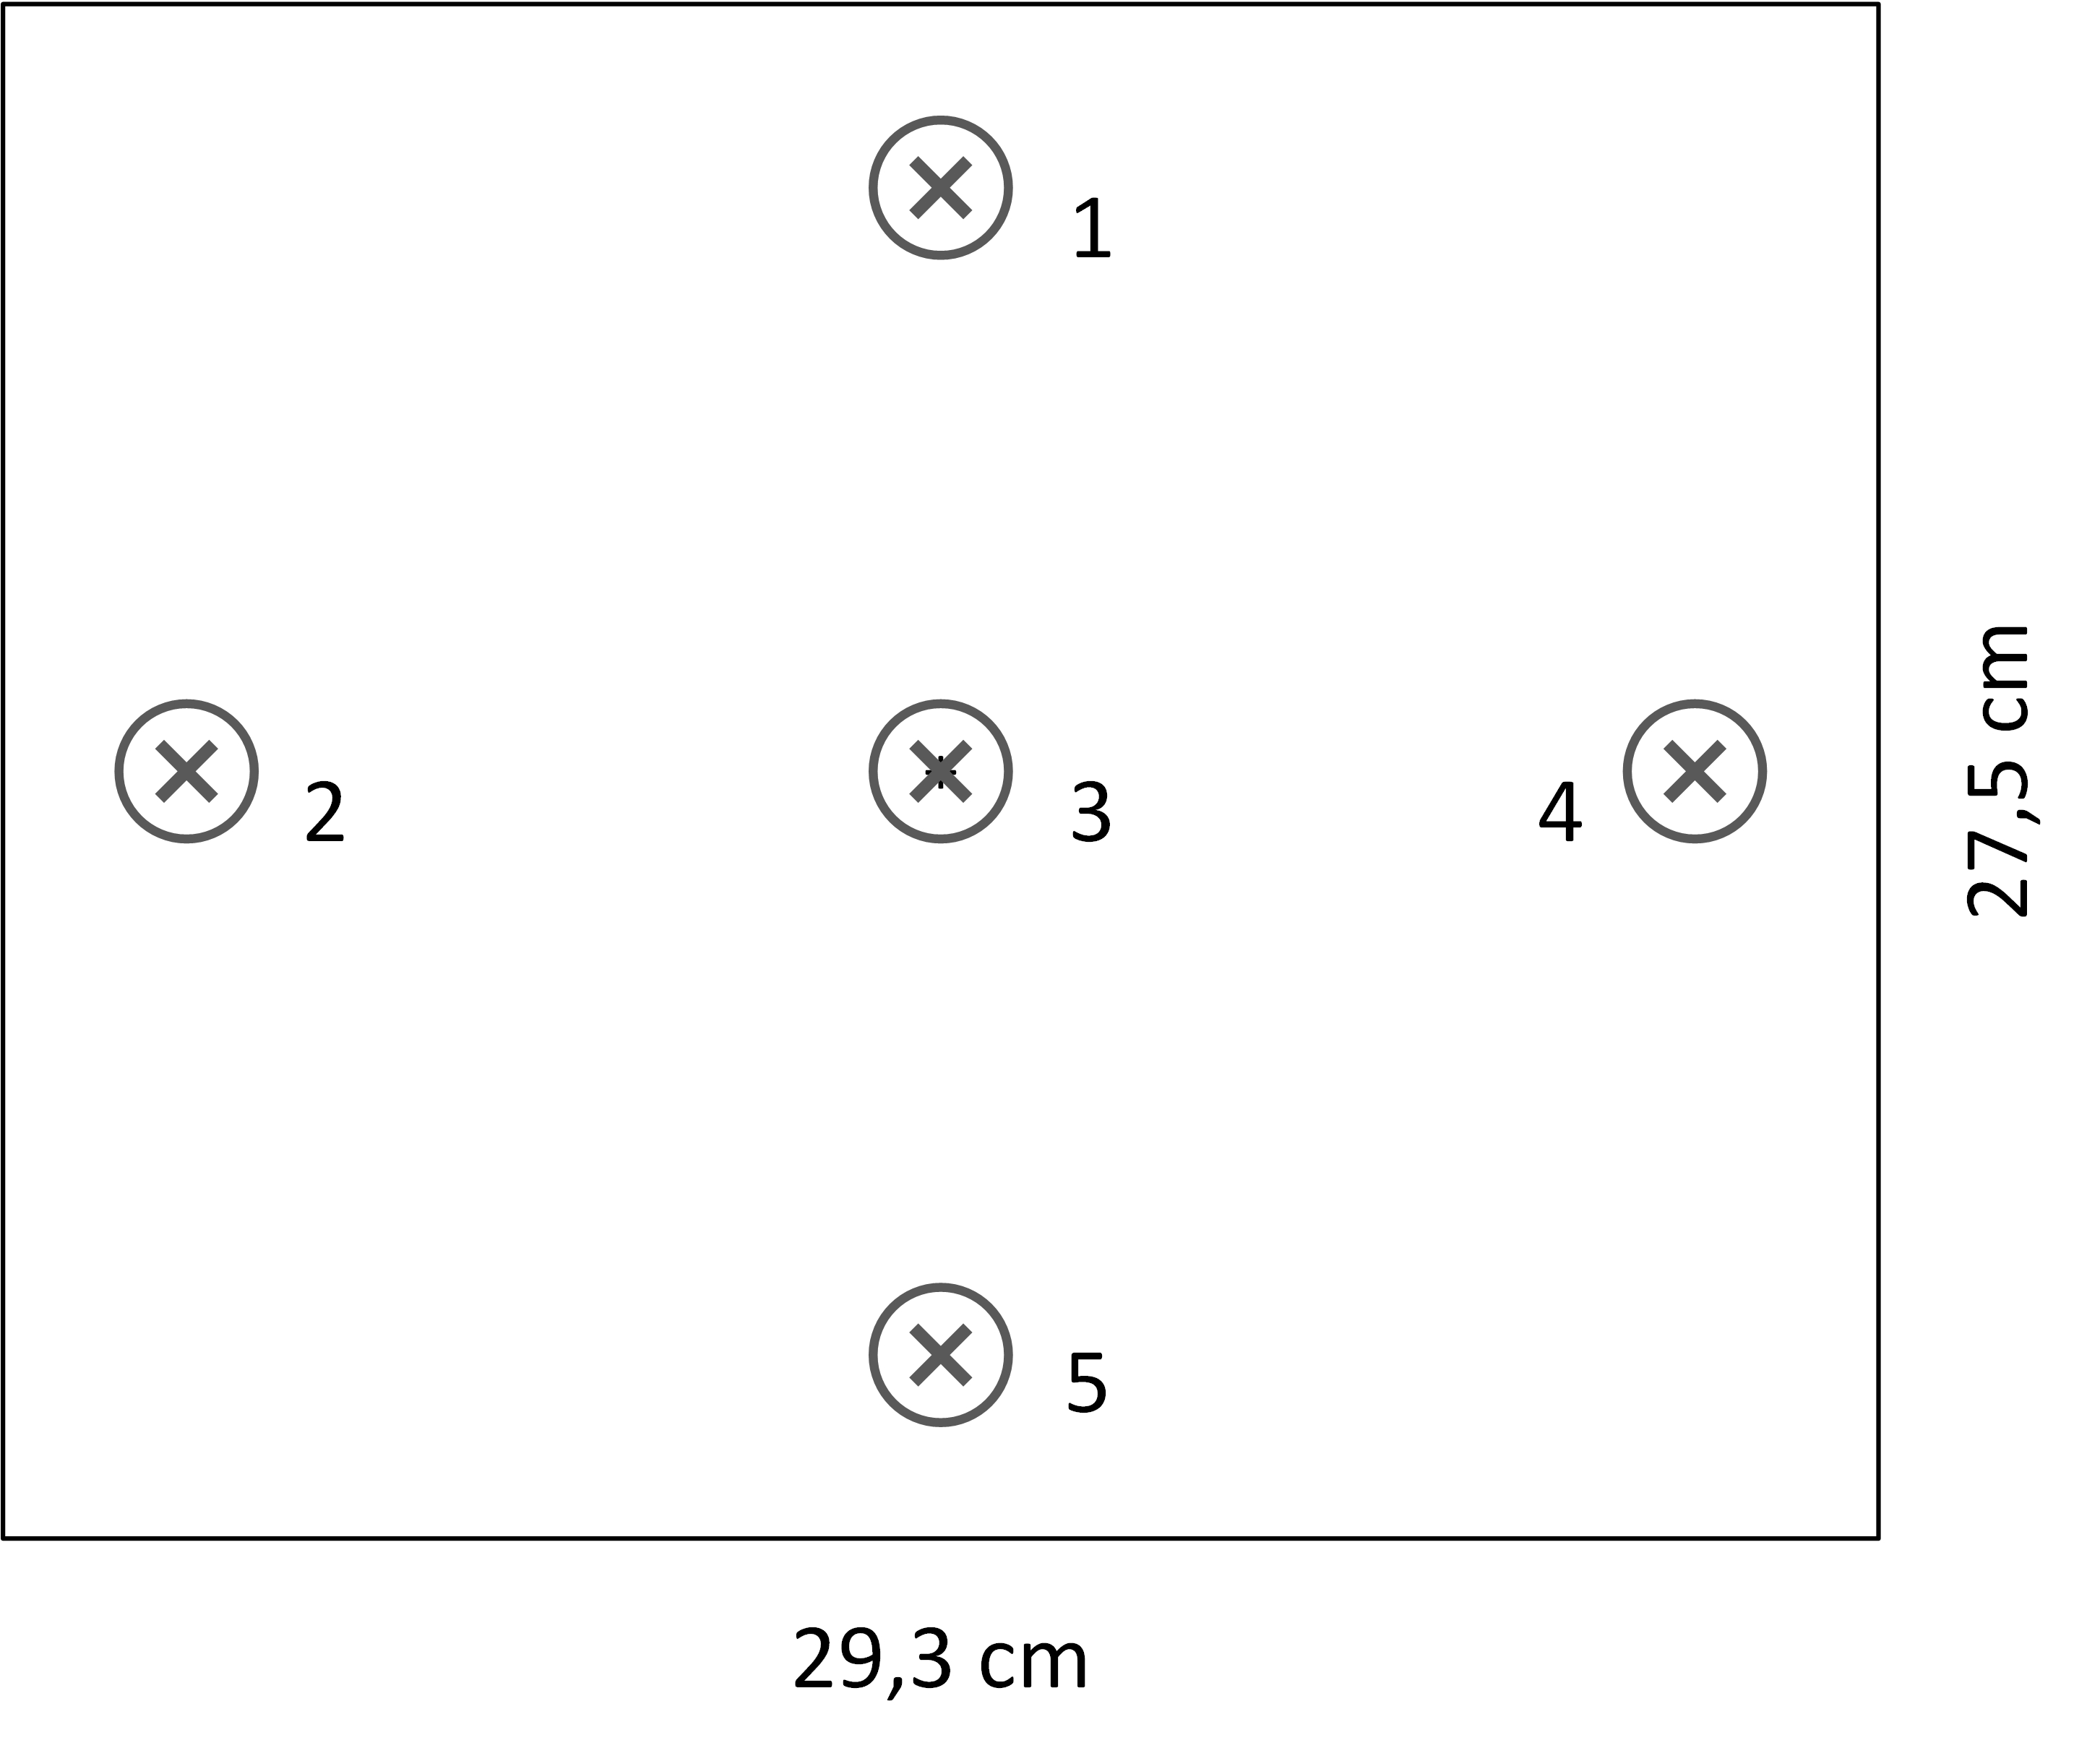
\includegraphics[width=0.4\textwidth]{img/luftschema}
	\caption{Skizze zur Messung der Luftgeschwindigkeiten und Abmaße des \mbox{luftgekoppelten} Verdampfers}
	\label{fig:luftschema}
\end{figure}
\FloatBarrier
%Ende

Ansonsten gilt für jede Messreihe, dass die entsprechenden Temperaturen der Ströme sensorisch gemessen und digital ausgegeben wurden. Die Kompressorleistung ließ sich dagegen für jede Messreihe analog mittels Zeiger des Drehpulsmesswerkes ablesen. Die Drücke in Kompressor und Kondensator wurden mittels Manometer aufgenommen und ebenfalls analog abgelesen.
Die Umgebungstemperatur, sowie der Umgebungsdruck wurden mit der bereitgestellten, anlagenunabhängigen  Barometer-Thermometer-Einheit analog abgelesen. 
